\clearpage
\section{Capacitance voltage editor}
Experimentally capacitance voltage (CV) measurements are a useful way to determine doping within a device. In OghmaNano CV measurements use a cut down version of frequency domain simulation tool described above.

\begin{figure}[H]
\centering
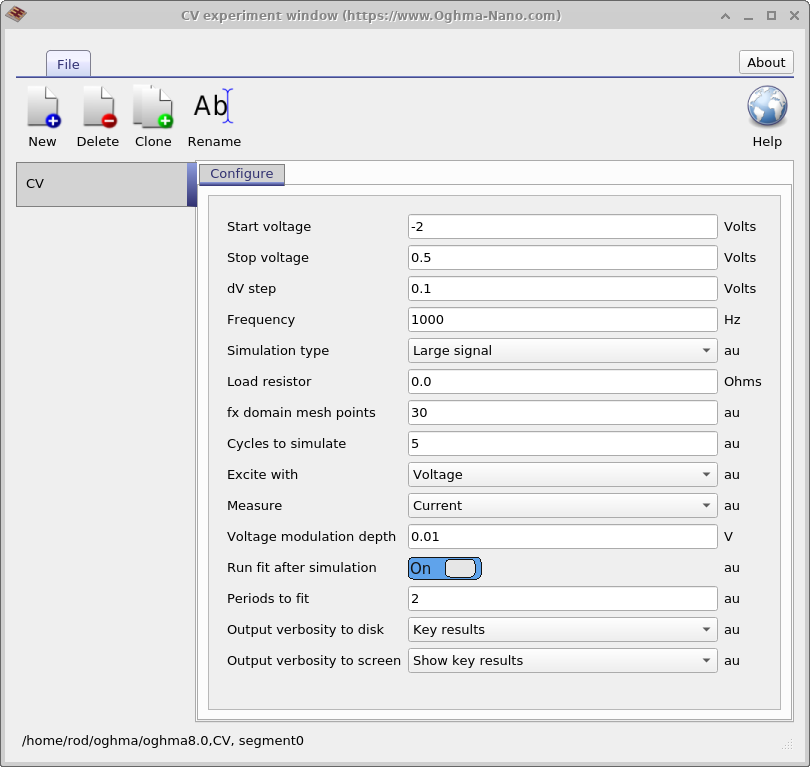
\includegraphics[width=0.7\textwidth,height=0.5\textwidth]{./images/sim_editors/cv.png}
\caption{The capacitance voltage editor}
\label{fig:cv_editor}
\end{figure}

\subsection{Outputs}

\begin{table}[H]
\begin{center}
\begin{tabular}{ |c|c| } 
 \hline
	File name 		& 	Description  \\ 
 \hline
	real\_imag.dat 		&	Re(i(fx)) v.s. Im(i(fx)) \\ 
	fx\_real.dat 		&	fx v.s. Re(i(fx)) \\ 
	fx\_imag.dat 		&	fx v.s. Im(i(fx)) \\ 
	cv.dat 				&	fx v.s. Capacitance \\ 
	cv2.dat 			&	fx v.s. $1/{Capacitance}^2$ \\ 
 \hline
\end{tabular}
\caption{Files produced by the CV simulation}
\label{tab:suns_jsc_output}
\end{center}
\end{table}
